% Chương 2

\chapter{CƠ SỞ LÝ THUYẾT DÙNG ĐỂ GIẢI QUYẾT BÀI TOÁN} 

\label{Chapter2}

\section{Mạng neural tích chập (Convolutional Neural Network - CNN)}

\subsection{Khái niệm}

Mạng neural tích chập (Convolutional Neural Network - CNN) là một loại mạng neural sử dụng trong lĩnh vực xử lý ảnh và nhận dạng. Nó sử dụng các lớp tích chập để trích xuất đặc trưng từ ảnh đầu vào và áp dụng các lớp kết nối đầy đủ để phân loại ảnh. 

\begin{figure}[h!]
	\centering
	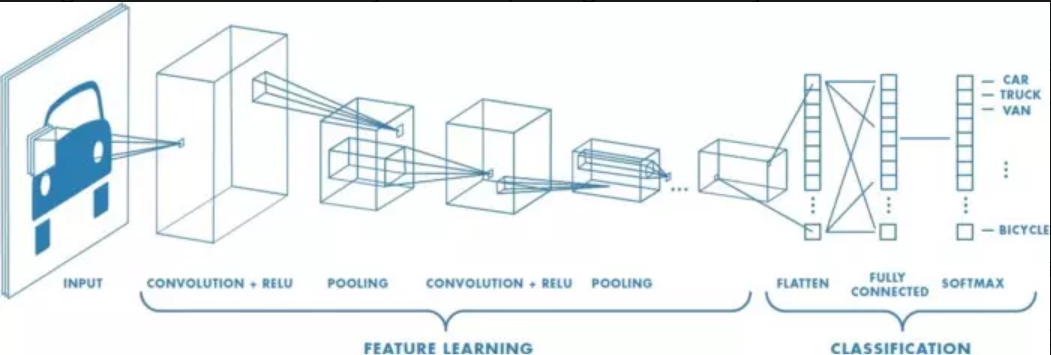
\includegraphics[width=0.8\textwidth]{CNN.png}
	\caption[Toàn bộ luồng CNN để xử lý hình ảnh đầu vào và phân loại các đối tượng dựa trên giá trị.]{Toàn bộ luồng CNN để xử lý hình ảnh đầu vào và phân loại các đối tượng dựa trên giá trị.}
	\label{fig:CNN} 
\end{figure}

Về kỹ thuật, mô hình CNN để training và kiểm tra, mỗi hình ảnh đầu vào sẽ chuyển nó qua 1 loạt các lớp tích chập với các bộ lọc (Kernel), tổng hợp lại các lớp được kết nối đầy đủ (Full Connected) và áp dụng hàm Softmax để phân loại đối tượng có giá trị xác suất giữa 0 và 1. Hình dưới đây là toàn bộ luồng CNN để xử lý hình ảnh đầu vào và phân loại các đối tượng dựa trên giá trị.

\begin{figure}[h!]
	\centering
	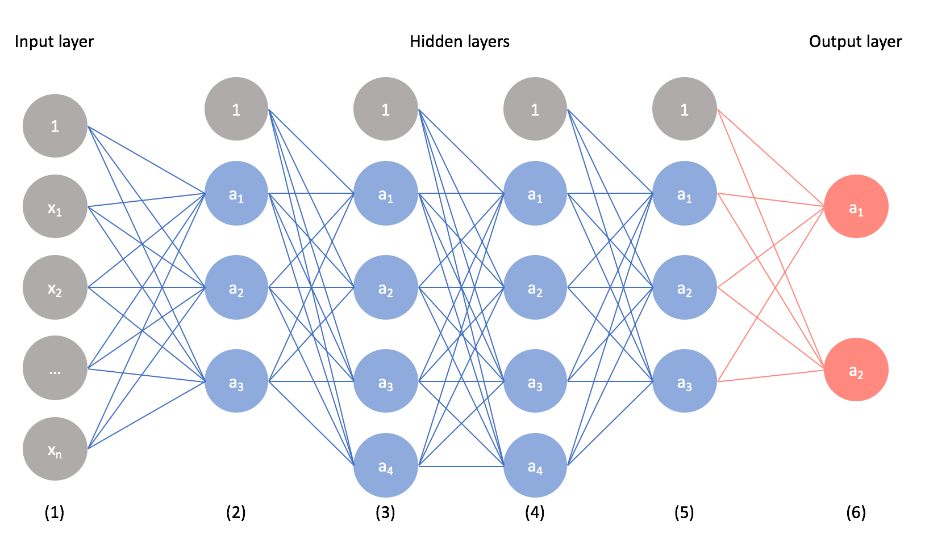
\includegraphics[width=0.7\textwidth]{anh2.png}
	\caption[Mô hình cấu trúc của mạng CNN.]{Mô hình cấu trúc của mạng CNN.}
	\label{fig:anh2} 
\end{figure}

\subsection{Feature trong CNN}

Các feature (đặc trưng) được sử dụng để trích xuất thông tin từ ảnh đầu vào. Các feature này được học tự động từ dữ liệu và được sử dụng để giảm thiểu số lượng thông tin cần xử lý trong quá trình huấn luyện mạng. 

Các feature này có thể là các đường cạnh, các vùng sáng tối, các đường cong và các đối tượng phức tạp hơn. 

Các feature này được trích xuất thông qua các bộ lọc tích chập và được kết hợp lại để tạo thành các feature maps, đóng vai trò quan trọng trong việc phân loại ảnh. Các feature maps này được đưa vào các lớp kết nối đầy đủ để phân loại ảnh đầu vào.

\subsection{Những lớp cơ bản của mạng CNN}

\subsubsection{Convolutional Layer}

Phần quan trọng nhất của toàn mạng CNN, các yếu tố quan trọng trong lớp Convolutional là: padding, stride, feature map và filter map.

\begin{itemize}
	\item Mạng CNN sử dụng filter để áp dụng vào các vùng của ma trận hình ảnh. Các filter map là các ma trận 3 chiều, bên trong đó là những tham số và chúng được gọi là parameters.
	
	\item Stride: dịch chuyển filter map theo từng pixel dựa vào các giá trị từ trái qua phải.
	
	\item Padding: Giá trị viền xung quanh của ma trận hình ảnh sẽ được gán các giá trị 0 để có thể tiến hành nhân tích chập ma trận mà không làm giảm kích thước ma trận ảnh ban đầu.
	
	\item Feature map: Biểu diễn kết quả sau mỗi lần feature map quét qua ma trận ảnh đầu vào. Sau mỗi lần quét thì lớp Convolutional sẽ tiến hành tính toán.
\end{itemize}

\begin{figure}[h!]
	\centering
	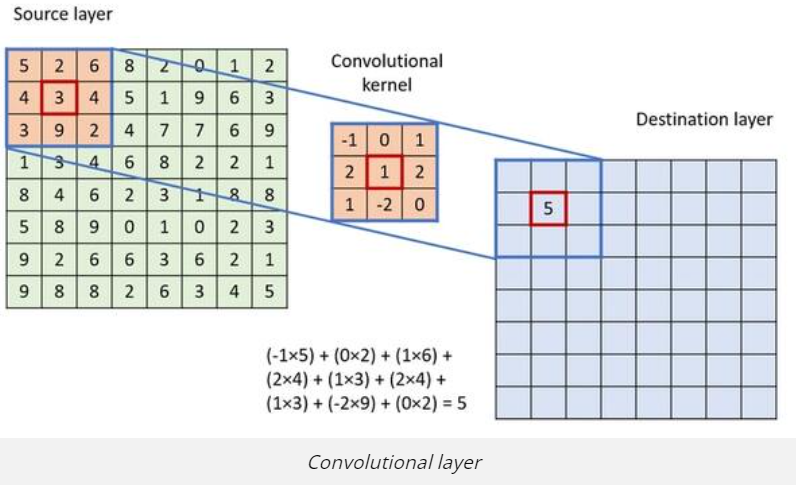
\includegraphics[width=0.7\textwidth]{convolution.png}
	\caption[Convolutional Layer.]{Convolutional Layer.}
	\label{fig:convolution} 
\end{figure}

\subsubsection{ReLU Layer}

Lớp ReLU là hàm kích hoạt trong mạng CNN, được coi là activation function. Nó có tác dụng mô phỏng những nơ ron có tỷ lệ truyền xung qua axon và hỗ trợ tính toán nhanh hơn.

Trong quá trình dùng hàm ReLU, chú ý đến việc tùy chỉnh learning rate và dead unit. Những lướp ReLU được dùng sau khi filter map được tính và áp dụng ReLU lên các giá trị của filter map.

\subsubsection{Pooling Layer}

Khi ma trận ảnh đầu vào có kích thước quá lớn, các lớp Pooling layer sẽ được đặt vào giữa những lớp Convolutional để làm giảm những parameters. Hai loại Pooling được sửu dụng phổ biến: Max pooling và Average.

\subsubsection{Fully Connected Layer}

Lớp có nhiệm vụ đưa ra kết quả sau khi 2 lớp Convolutional và Pooling đã nhận được ảnh truyền, khi này, ta sẽ thu được một model đọc được thông tin của ảnh.

\subsection{Kiến trúc của mạng CNN}

Mạng CNN là tập hợp những Convolutional layer xếp chồng lên nhau, đồng thời mạng sử dụng những hàm như ReLU và Tanh để kích hoạt các trọng số trong các node. Các lớp này sau khi qua các hàm activation sẽ có trọng số trong những node và có thể tạo ra những thông tin trừu tượng hơn đến với các lớp kế tiếp trong mạng.  

Cấu trúc cơ bản của một mô hình CNN:

\begin{itemize}
	\item Local receptive: Lớp này sử dụng để tách lọc dữ liệu, thông tin hình ảnh để từ đó có thể lựa chọn các vùng có giá trị sử dụng hiệu quả cao nhất.
	
	\item Shared weights field: Lớp này hỗ trợ làm giảm các tham số đến mức tối thiểu trong mạng CNN. Trong từng lớp convolution sẽ chứa các feature map riêng và từng feature thì sẽ có khả năng phát hiện một vài feature trong hình ảnh.
	
	\item Pooling layer: Lớp cuối cùng và sử dụng để làm đơn giản các thông tin output. Sau khi tính toán xong và quét qua các layer trong mạng thì pooling layer sẽ được dùng để lược bỏ các thông tin không hữu ích.
\end{itemize}
\section{Mạng hồi quy RNN}
Con người không bắt đầu suy nghĩ của họ từ đầu tại tất cả các thời điểm. Cũng như bạn đang đọc bài viết này, bạn hiểu mỗi chữ ở đây dựa vào từ bạn đã hiểu các chữ trước đó chứ không phải là đọc tới đâu ném hết đi tới đó, rồi lại bắt đầu suy nghĩ lại từ đầu tới chữ bạn đang đọc. Tức là tư duy đã có một bộ nhớ để lưu lại những gì diễn ra trước đó.

Tuy nhiên các mô hình mạng nơ-ron truyền thống thì không thể làm được việc đó, đó có thể coi là một khuyết điểm chính của mạng nơ-ron truyền thống. Ví dụ, bạn muốn phân loại các bối cảnh xảy ra ở tất cả các thời điểm trong một bộ phim, thì đúng là không rõ làm thế nào để có thể hiểu được một tình huống trong phim mà lại phụ thuộc vào các tình huống trước đó nếusử dụng các mạng nơ-ron truyền thống.

Mạng nơ-ron hồi quy (Recurrent Neural Network) sinh ra để giải quyết vấn đề đó. Mạng này chứa các vòng lặp bên trong cho phép thông tin có thể lưu lại được.
\begin{figure}[h!]
	\centering
	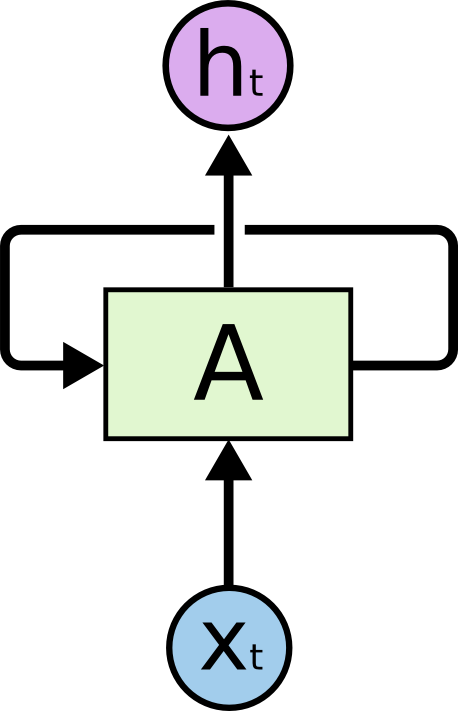
\includegraphics[width=0.7\textwidth]{Figures/RNN-rolled.png}
	\caption[Một đoạn RNN.]{Một đoạn RNN.}
	\label{fig:RNN-rolled.png} 
\end{figure}
Hình vẽ trên mô tả một đoạn của mạng nơ-ron hồi quy A với đầu vào là \( x_{t} \) và đầu ra là \( h_{t} \).Một vòng lặp cho phép thông tin có thể được truyền từ bước này qua bước này qua bước khác của mạng nơ-ron.

Các vòng lặp này khiến cho mạng nơ-ron hồi quy trông có vẻ khó hiểu. Tuy nhiên, nếu bạn để ý một chút thì nó không khác mấy so với các mạng nơ-ron thuần. Một mạng nơ-ron hồi quy có thể được coi là nhiều bản sao chép của cùng một mạng, trong đó mỗi đầu ra của mạng này là đầu vào của một mạng sao chép khác. Nói thì hơi khó hiểu, nhưng bạn hãy xem hình mô tả sau:
\begin{figure}[h!]
	\centering
	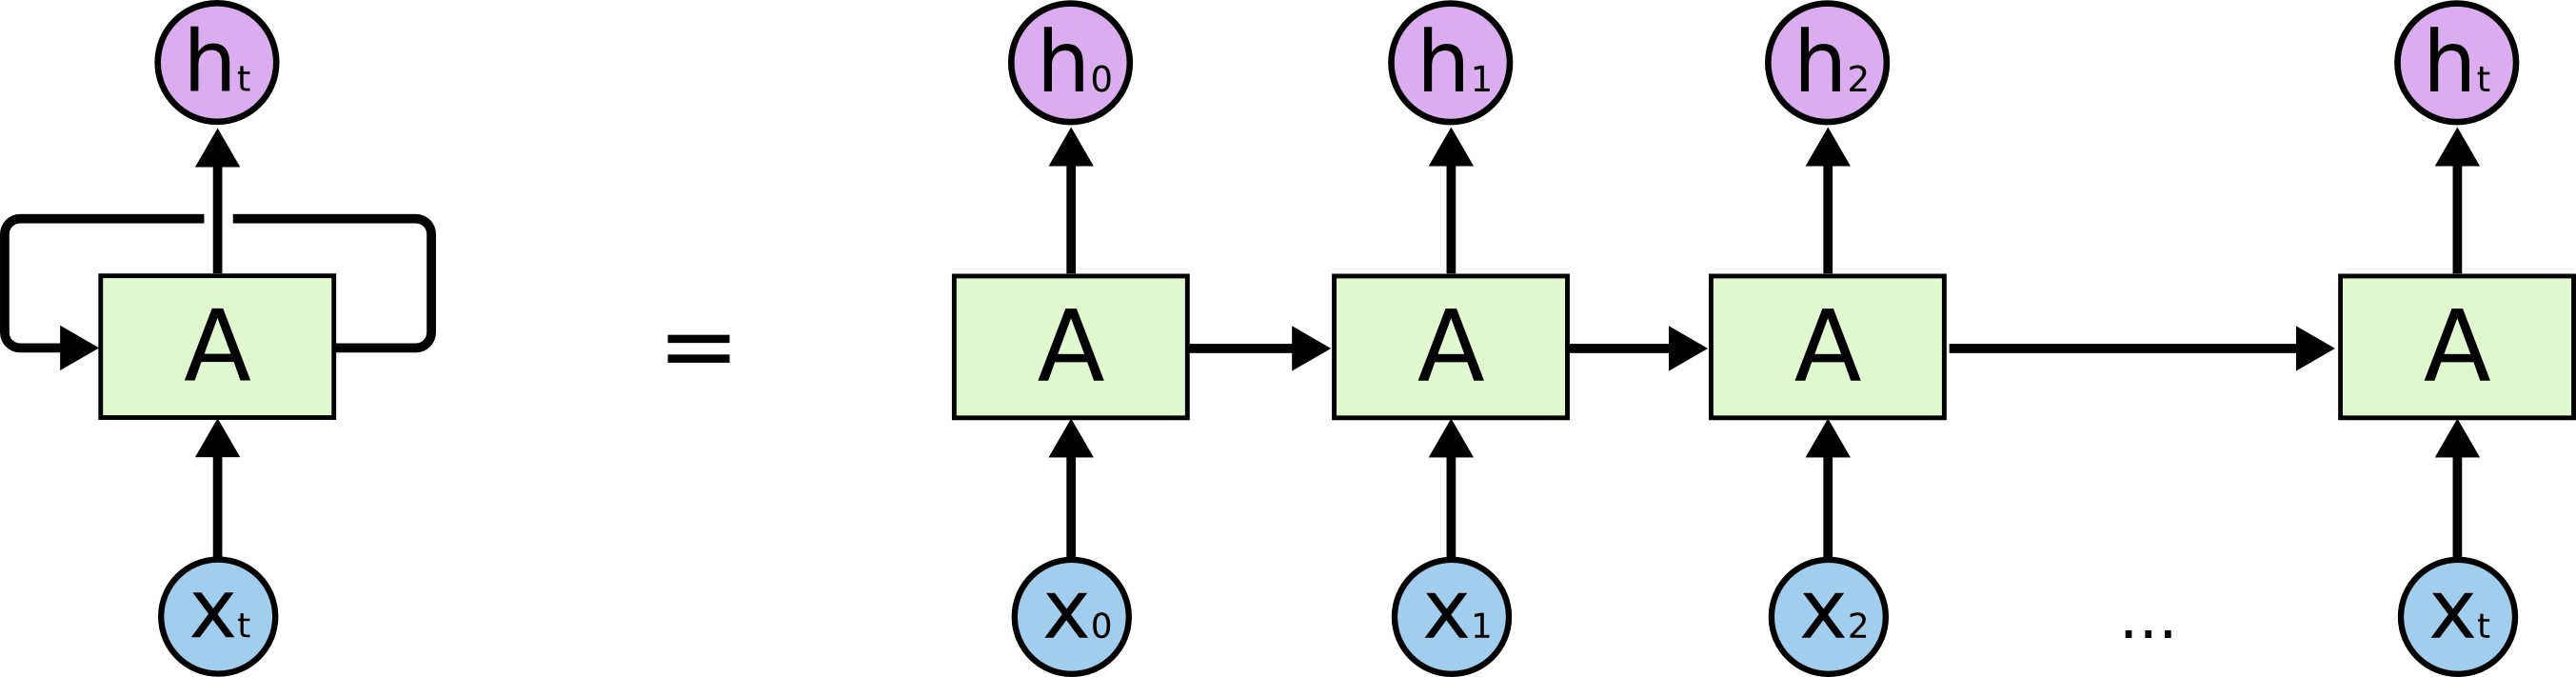
\includegraphics[width=0.7\textwidth]{Figures/RNN-unrolled.png}
	\caption[Mạng RNN.]{Mạng RNN.}
	\label{fig:RNN-unrolled.png} 
\end{figure}
Chuỗi lặp lại các mạng này chính là phân giải của mạng nơ-ron hồi quy, các vòng lặp khiến chúng tạo thành một chuỗi danh sách các mạng sao chép nhau. Bạn có thấy nó khác gì một mạng nơ-ron thuần không? Không khác gì phải không? Các nút của mạng vẫn nhận đầu vào và có đầu ra hệt như mạng nơ-ron thuần.

Trong vài năm gần đây, việc ứng dụng RNN đã đưa ra được nhiều kết quả không thể tin nổi trong nhiều lĩnh vực: nhận dạng giọng nói, mô hình hóa ngôn ngữ, dịch máy, mô tả ảnh,… Danh sách vẫn còn đang được mở rộng tiếp. Anh Andrej Karpathy đã đề cập tới một số kêt quả mà RNN mang lại tại bài viết này, nên tôi sẽ không bàn luận thêm nữa. Nhưng tôi vẫn muốn thốt lên rằng chúng thật là quá tuyệt vời.

Đằng sau sự thành công này chính là sự đóng góp của LSTM. LSTM là một dạng đặc biệt của mạng nơ-ron hồi quy, với nhiều bài toán thì nó tốt hơn mạng hồi quy thuần. Hầu hết các kết quả thú vị thu được từ mạng RNN là được sử dụng với LSTM. Trong bài viết này, ta sẽ cùng khám phá xem mạng LSTM là cái gì nhé.
\section{Mạng LSTM}
Mạng nơ-ron LSTM( Long Short-Term Memory là một loại mạng nơ ron hồi quy RNN được thiết kế đặc biệt để giải quyết vấn đề biến mất đường hồi quy (vanishing grandient) trong việc xử lý chuỗi liên tục . Biến mất đường hồi quy là hiện tượng khi gradient trong quá trình lan truyền ngược giảm đi rất nhanh , gây khó khăn trong việc  học các phụ thuộc xa trong dữ liệu chuỗi . LSTM đã được giới thiệu vào năm 1997 bởi Sep Hochreiter và Jurgen Schmidhuber và từ đó trở thành một trong những mô hình RNN phổ biến nhất và hiệu quả nhất . 

\subsubsection{Tổng quan về LSTM}

\begin{figure}[h!]
	\centering
	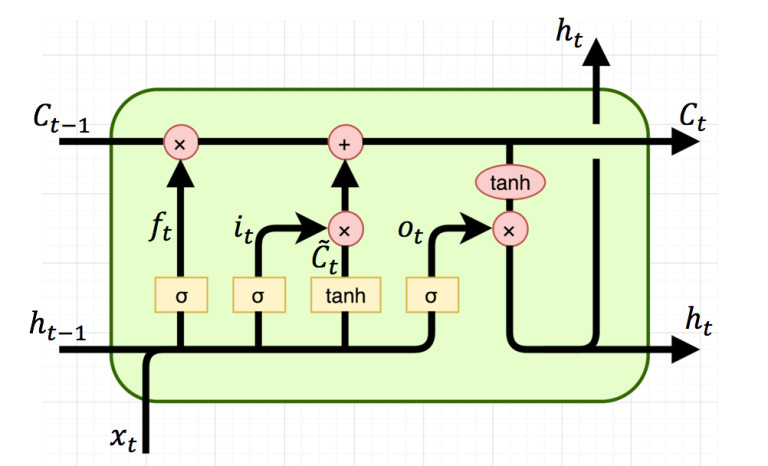
\includegraphics[width=0.7\textwidth]{Figures/lstm-all.jpg}
	\caption[Mô hình LSTM.]{Mô hình LSTM.}
	\label{fig:lstm-all.jpg} 
\end{figure}
LSTM được thiết kế để tránh được vấn đề phụ thuộc xa (long-term dependency). Việc nhớ thông tin trong suốt thời gian dài là đặc tính mặc định của chúng, chứ ta không cần phải huấn luyện nó để có thể nhớ được. Tức là ngay nội tại của nó đã có thể ghi nhớ được mà không cần bất kì can thiệp nào.

Mọi mạng hồi quy đều có dạng là một chuỗi các mô-đun lặp đi lặp lại của mạng nơ-ron. Với mạng RNN chuẩn, các mô-dun này có cấu trúc rất đơn giản, thường là một tầng tanh
\begin{figure}[h!]
	\centering
	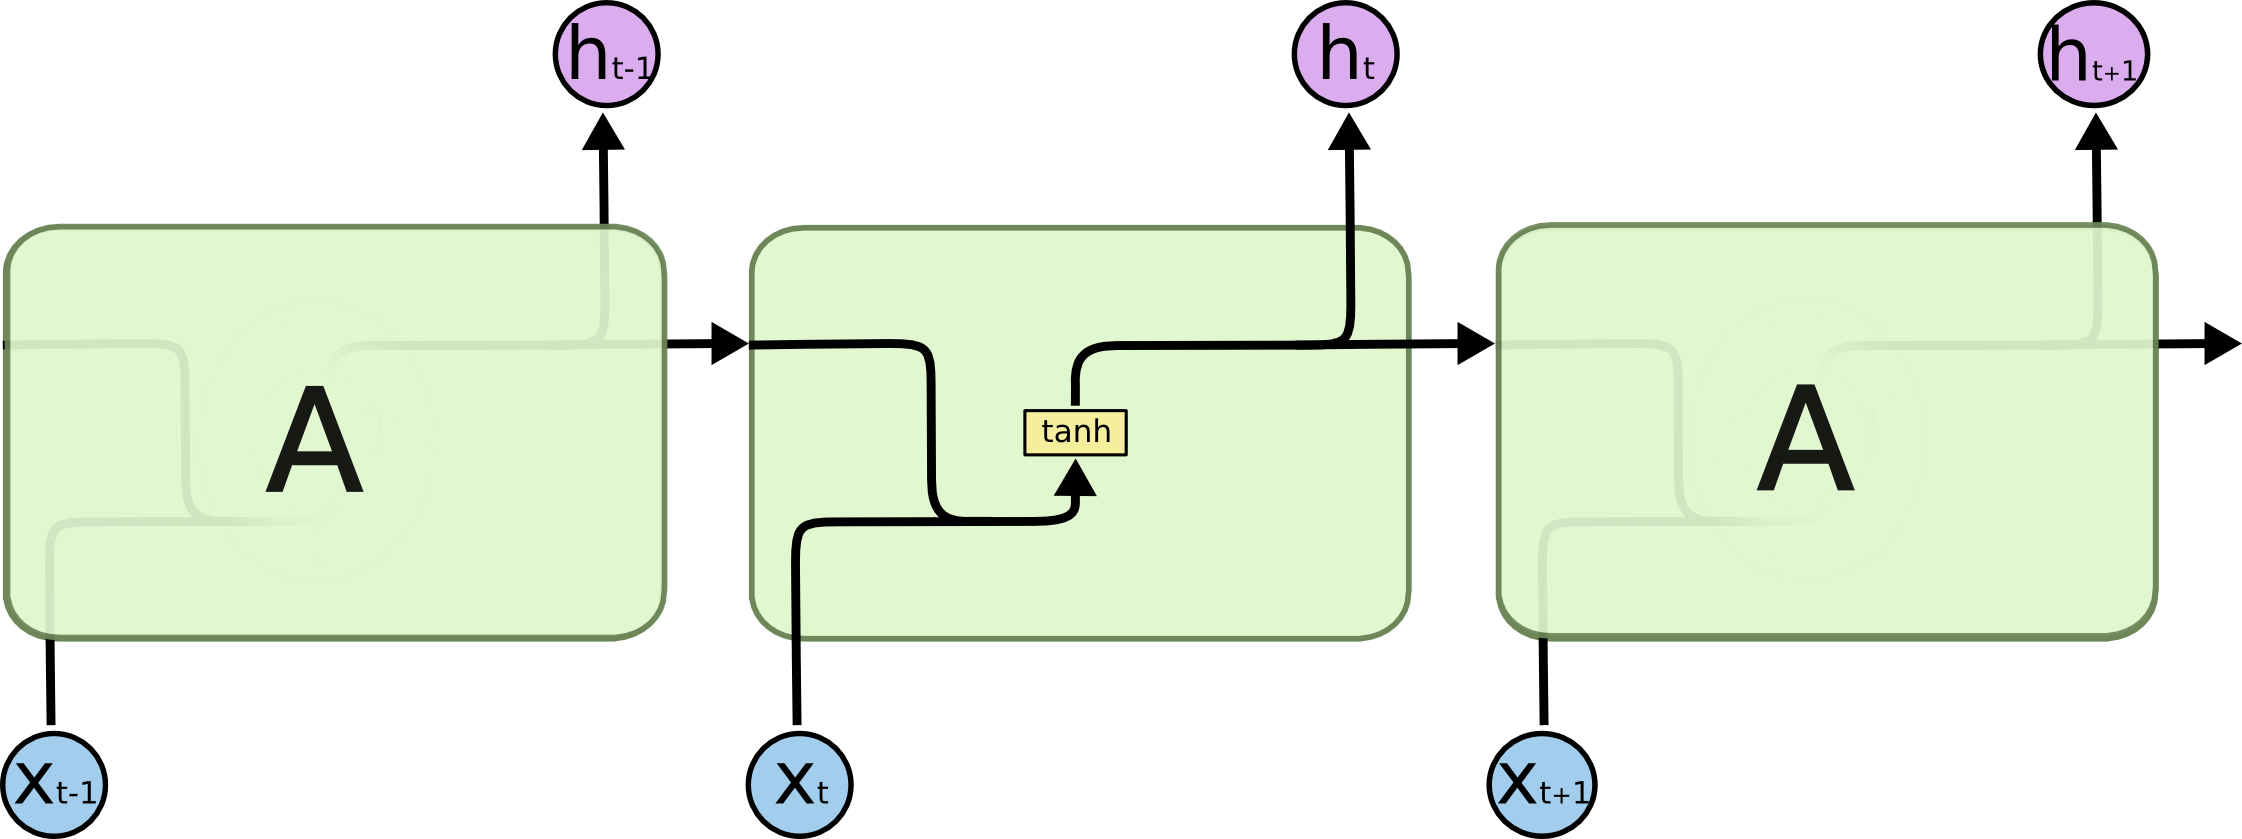
\includegraphics[width=0.7\textwidth]{LSTM3-SimpleRNN.png}
	\caption[Mạng RNN chuẩn.]{Mạng RNN chuẩn.}
	\label{fig:LSTM3-SimpleRNN.png} 
\end{figure}
LSTM cũng có kiến trúc dạng chuỗi như vậy, nhưng các mô-đun trong nó có cấu trúc khác với mạng RNN chuẩn. Thay vì chỉ có một tầng mạng nơ-ron, chúng có tới 4 tầng tương tác với nhau một cách rất đặc biệt.

\begin{figure}[h!]
	\centering
	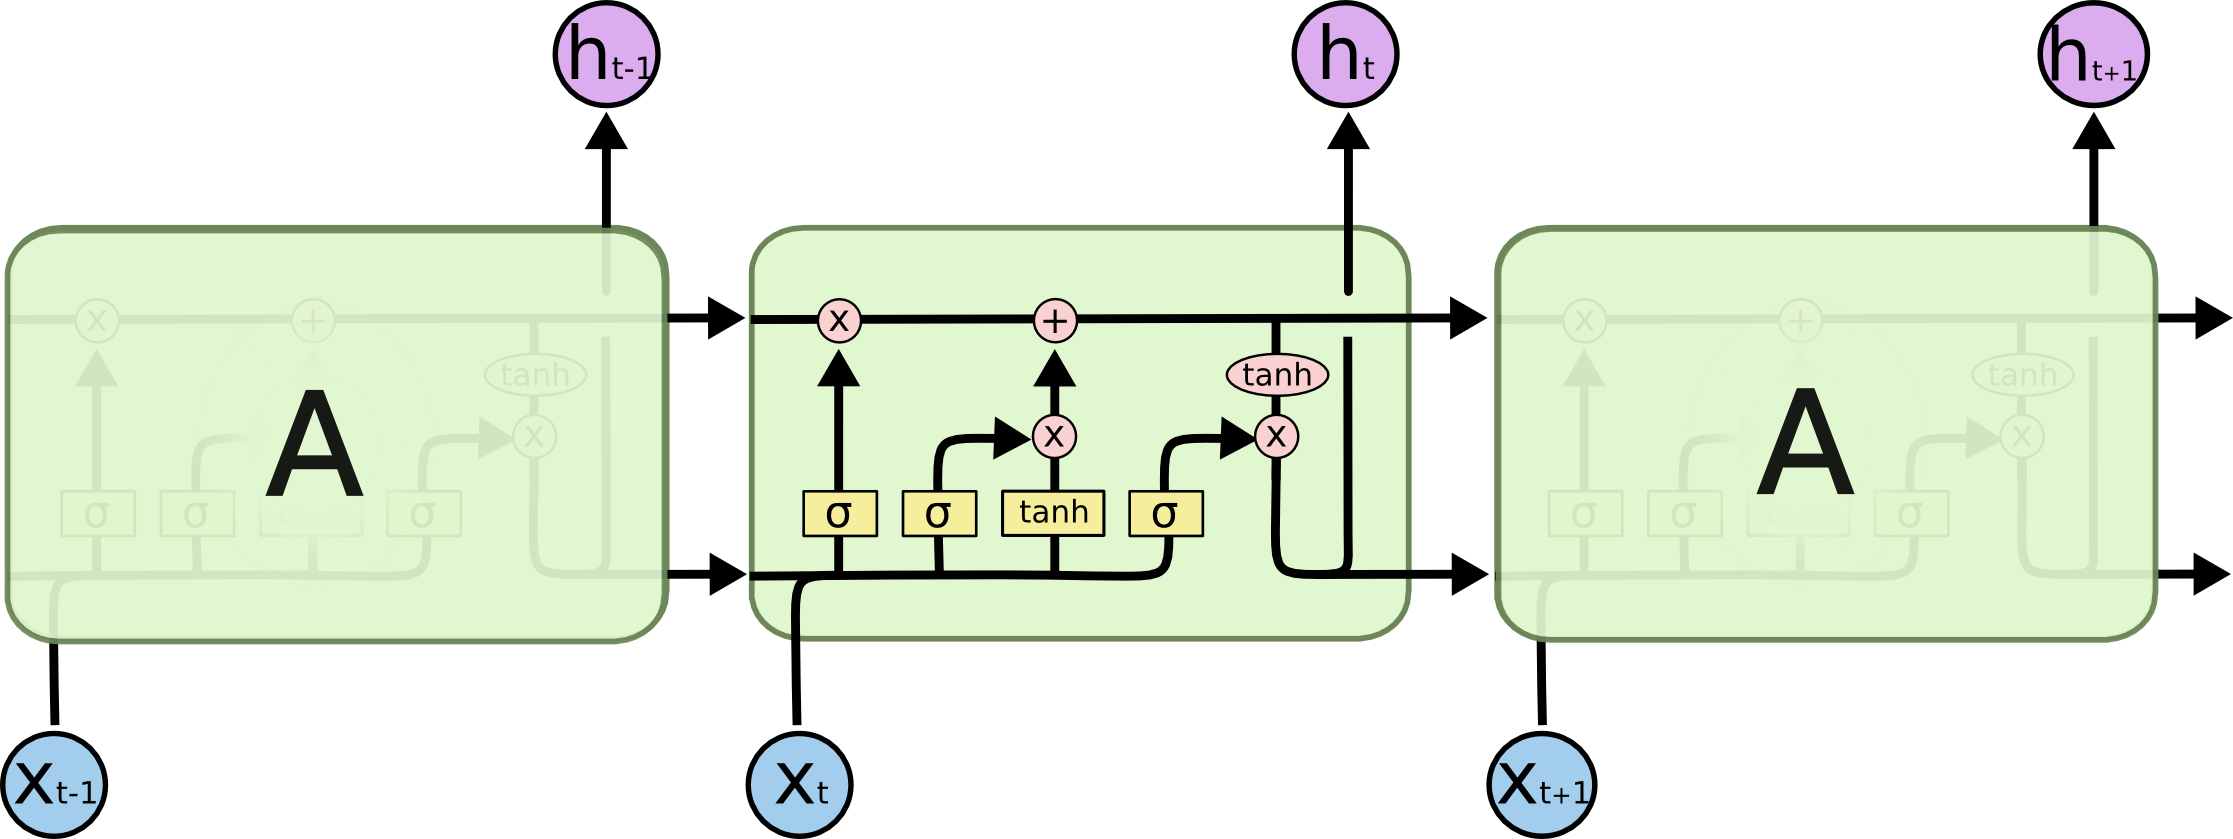
\includegraphics[width=0.7\textwidth]{Figures/LSTM3-chain.png}
	\caption[Mạng LSTM.]{Mạng LSTM.}
	\label{fig:LSTM.png} 
\end{figure}
\subsubsection{Ý tưởng cốt lõi của LSTM}
Chìa khóa của LSTM là trạng thái tế bào (cell state) - chính đường chạy thông ngang phía trên của sơ đồ hình vẽ.

Trạng thái tế bào là một dạng giống như băng truyền. Nó chạy xuyên suốt tất cả các mắt xích (các nút mạng) và chỉ tương tác tuyến tính đôi chút. Vì vậy mà các thông tin có thể dễ dàng truyền đi thông suốt mà không sợ bị thay đổi.

\begin{figure}[h!]
	\centering
	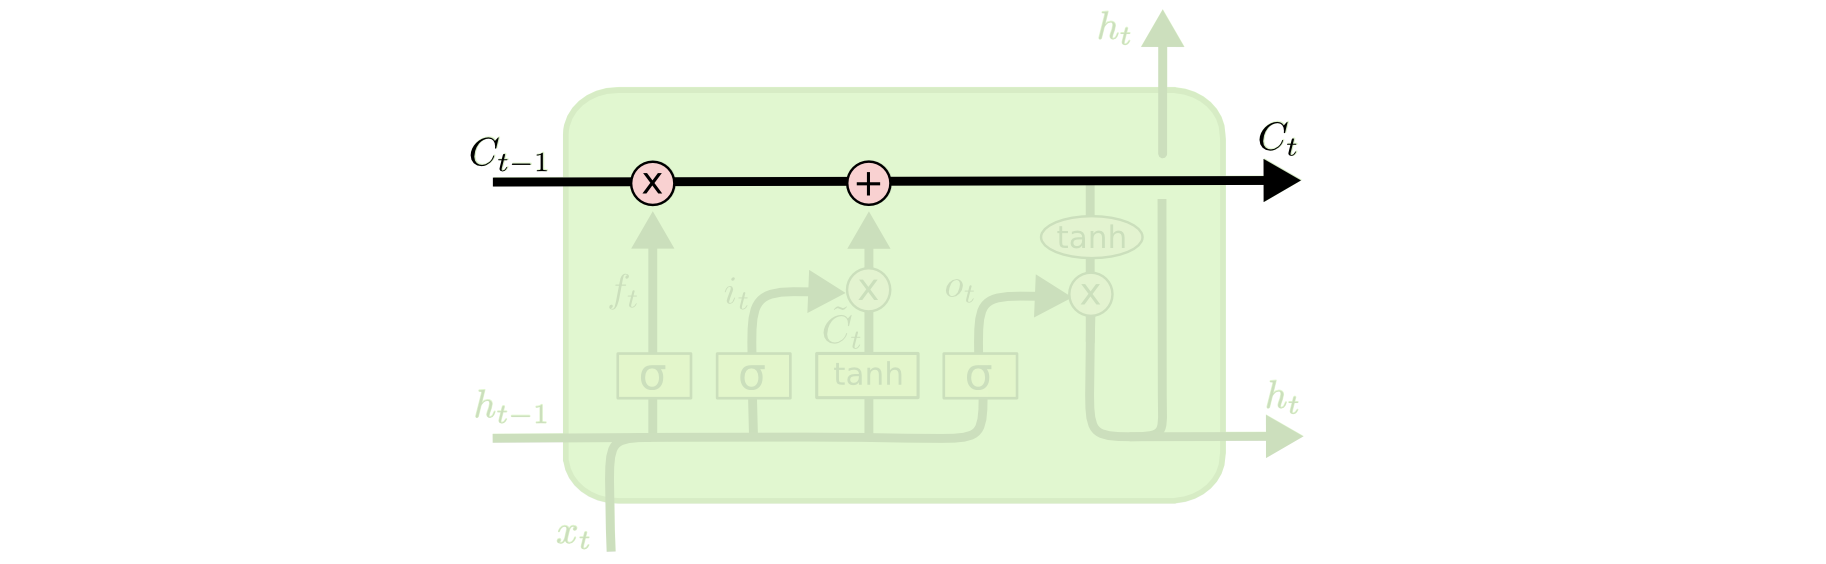
\includegraphics[width=0.7\textwidth]{Figures/LSTM3-C-line.png}
	\caption[Mạng LSTM line.]{Mạng LSTM line.}
	\label{fig:LSTM3-C-line.png} 
\end{figure}
LSTM có khả năng bỏ đi hoặc thêm vào các thông tin cần thiết cho trạng thái tế báo, chúng được điều chỉnh cẩn thận bởi các nhóm được gọi là cổng (gate).

Các cổng là nơi sàng lọc thông tin đi qua nó, chúng được kết hợp bởi một tầng mạng sigmoid và một phép nhân.

\begin{figure}[h!]
	\centering
	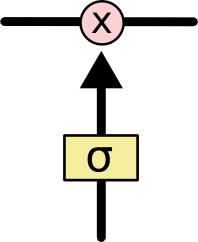
\includegraphics[width=0.7\textwidth]{Figures/LSTM3-gate.png}
	\caption[Cổng Gate.]{Cổng Gate.}
	\label{fig:LSTM3-gate.png} 
\end{figure}
Tầng sigmoid sẽ cho đầu ra là một số trong khoản [0,1], mô tả có bao nhiêu thông tin có thể được thông qua. Khi đầu ra là 0 thì có nghĩa là không cho thông tin nào qua cả, còn khi là 1 thì có nghĩa là cho tất cả các thông tin đi qua nó.
Một LSTM gồm có 3 cổng như vậy để duy trì và điều hành trạng thái của tế bào.
\subsubsection{Thành phần của LSTM}


\subsubsection{Bên trong LSTM}

\begin{itemize}
    \item Bước đầu tiên của LSTM là quyết định xem thông tin nào cần bỏ đi từ trạng thái tế bào. Quyết định này được đưa ra bởi tầng sigmoid - gọi là “tầng cổng quên” (forget gate layer) . Nó sẽ lấy đầu vào là  \( h_{t-1} \) và \( x_{t} \) rồi đưa kết quả là một trong khoảng [0,1] cho mỗi trạng thái tế bào \( C_{t-1} \) . Đầu ra là 1 thể hiện rằng nó giữ toàn bộ thông tin lại . còn 0 chỉ là toàn bộ thông tin sẽ bị bỏ đi 
    \begin{figure}[h!]
	\centering
	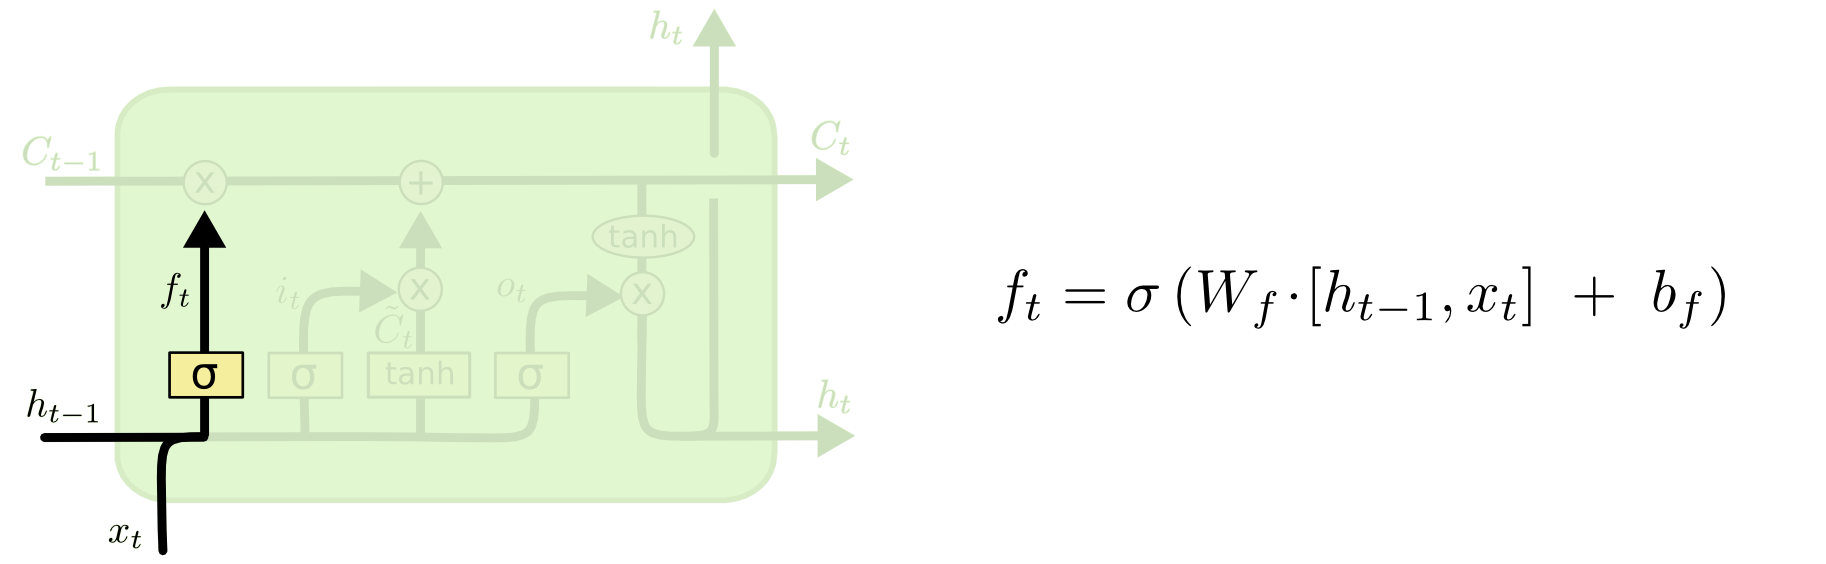
\includegraphics[width=0.7\textwidth]{Figures/LSTM3-focus-f.png}
	\caption[Forget Gate.]{Forget Gate.}
	\label{LSTM3-focus-f.png} 
\end{figure}
    \item Bước tiếp theo là quyết định xem thông tin mới nào ta sẽ lưu vào trạng thái tế bào. Việc này gồm 2 phần. Đầu tiên là sử dụng một tầng sigmoid được gọi là “tầng cổng vào” (input gate layer) để quyết định giá trị nào ta sẽ cập nhập. Tiếp theo là một tầng tanh để tạo ra một vec-to cho giá trị mới \( C_{t} \) nhằm thêm vào cho trạng thái. Trong bước tiếp theo, ta sẽ kết hợp 2 giá trị đó lại để tạo ra một cập nhập cho trạng thái.
    \begin{figure}[h!]
	\centering
	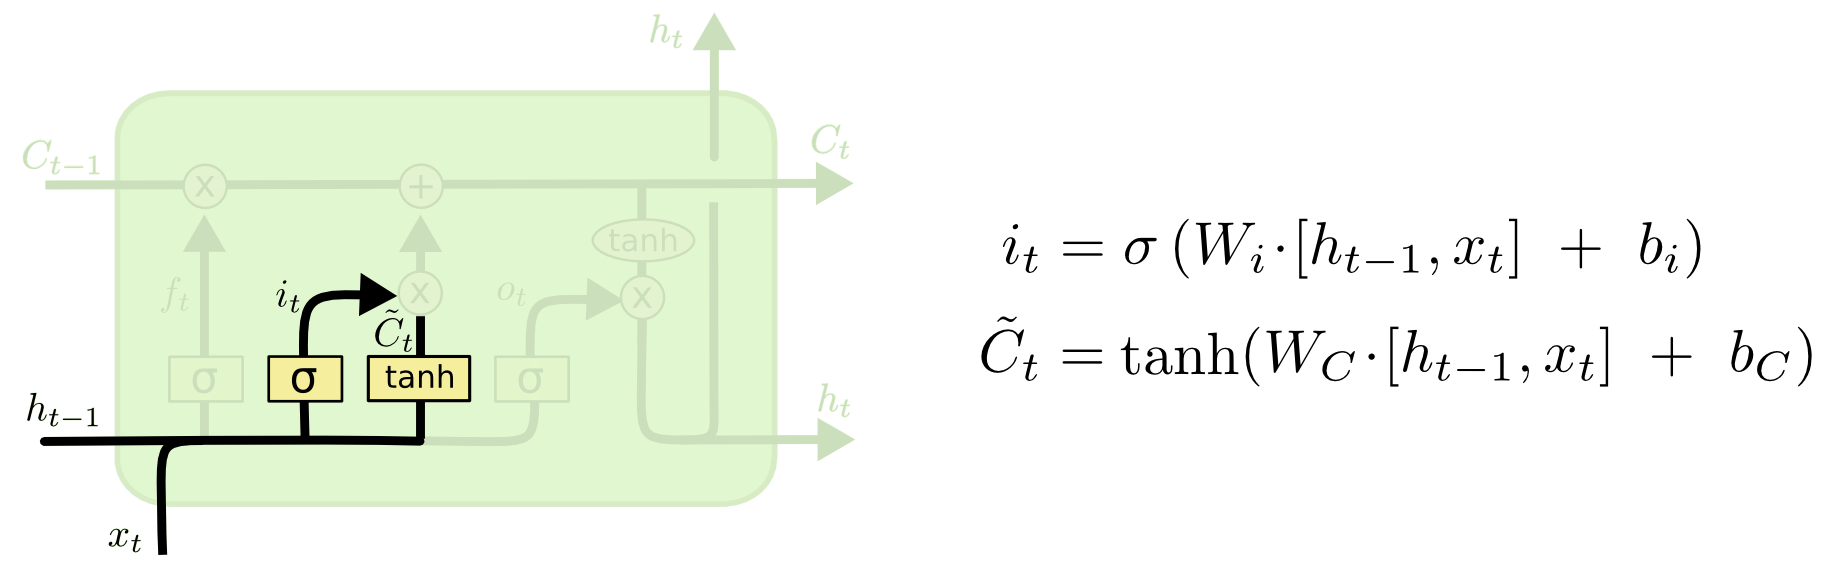
\includegraphics[width=0.7\textwidth]{Figures/LSTM3-focus-i.png}
	\caption[Input Gate.]{Input Gate.}
	\label{LSTM3-focus-i.png} 
\end{figure}
    \item Sau đó , LSTM cập nhật trạng thái của Cell State \( C_{t-1} \) thành trạng thái mới \( C_{t} \) bằng cách kết hợp thông tin mới và thông tin cũ . Ta sẽ nhân trạng thái cũ với \( f_{t} \) để bỏ đi những thông tin ta quyết định quên lúc trước. Sau đó cộng thêm \( i_{t} \) * \( C_{t} \)  Trạng thái mơi thu được này phụ thuộc vào việc ta quyết định cập nhập mỗi giá trị trạng thái ra sao.
    \begin{figure}[h!]
	\centering
	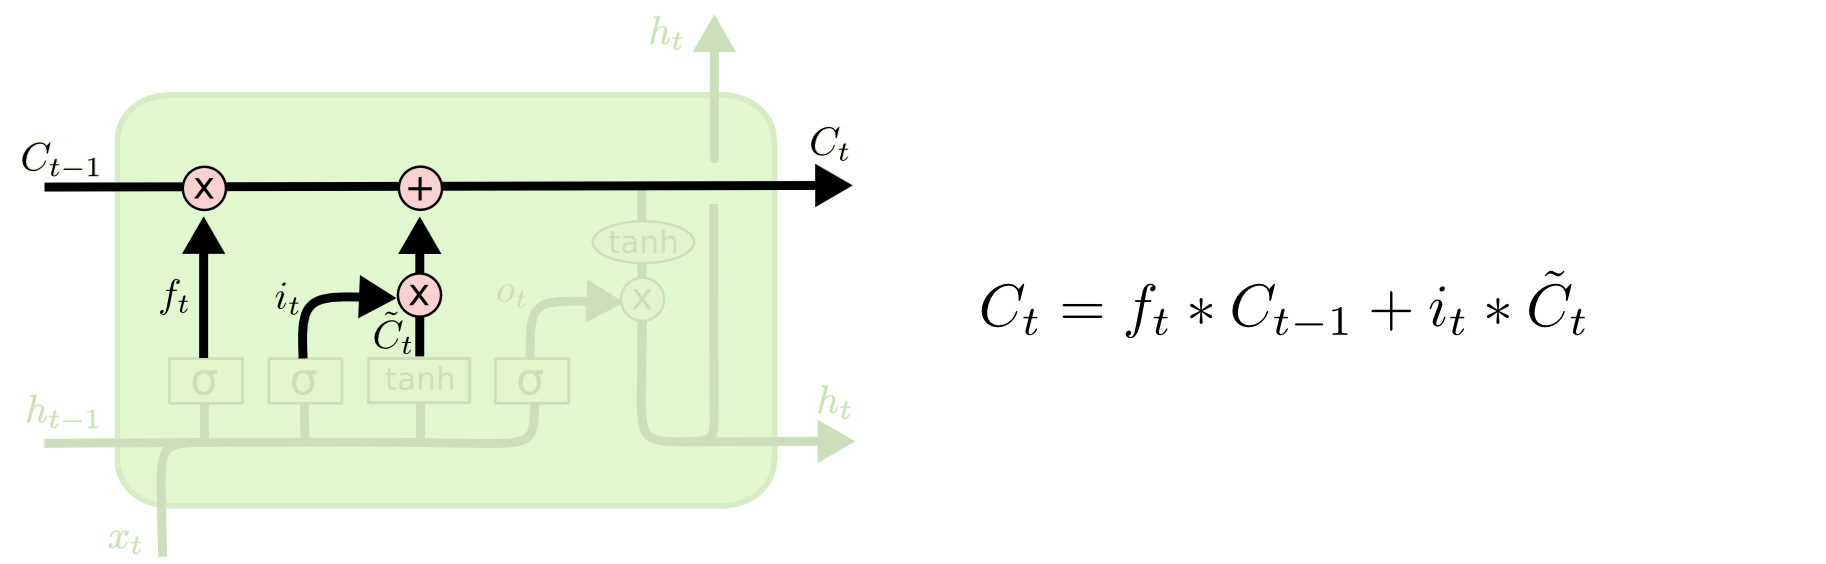
\includegraphics[width=0.7\textwidth]{Figures/LSTM3-focus-C.png}
	\caption[Cell Gate.]{Cell Gate.}
	\label{LSTM3-focus-C.png} 
\end{figure}
    \item Cuối cùng ,LSTM tính toán giá trị của cổng đầu ra và sử dụng nó để tính toán đầu ra của đơn vị LSTM hiện tại và truyền trạng thái ẩn tới đơn vị LSTM tiếp theo trong chuỗi .Đầu tiên, ta chạy một tầng sigmoid để quyết định phần nào của trạng thái tế bào ta muốn xuất ra. Sau đó, ta đưa nó trạng thái tế bảo qua một hàm tanh để co giá trị nó về khoảng [-1,1],và nhân nó với đầu ra của cổng sigmoid để được giá trị đầu ra ta mong muốn.
    \begin{figure}[h!]
	\centering
	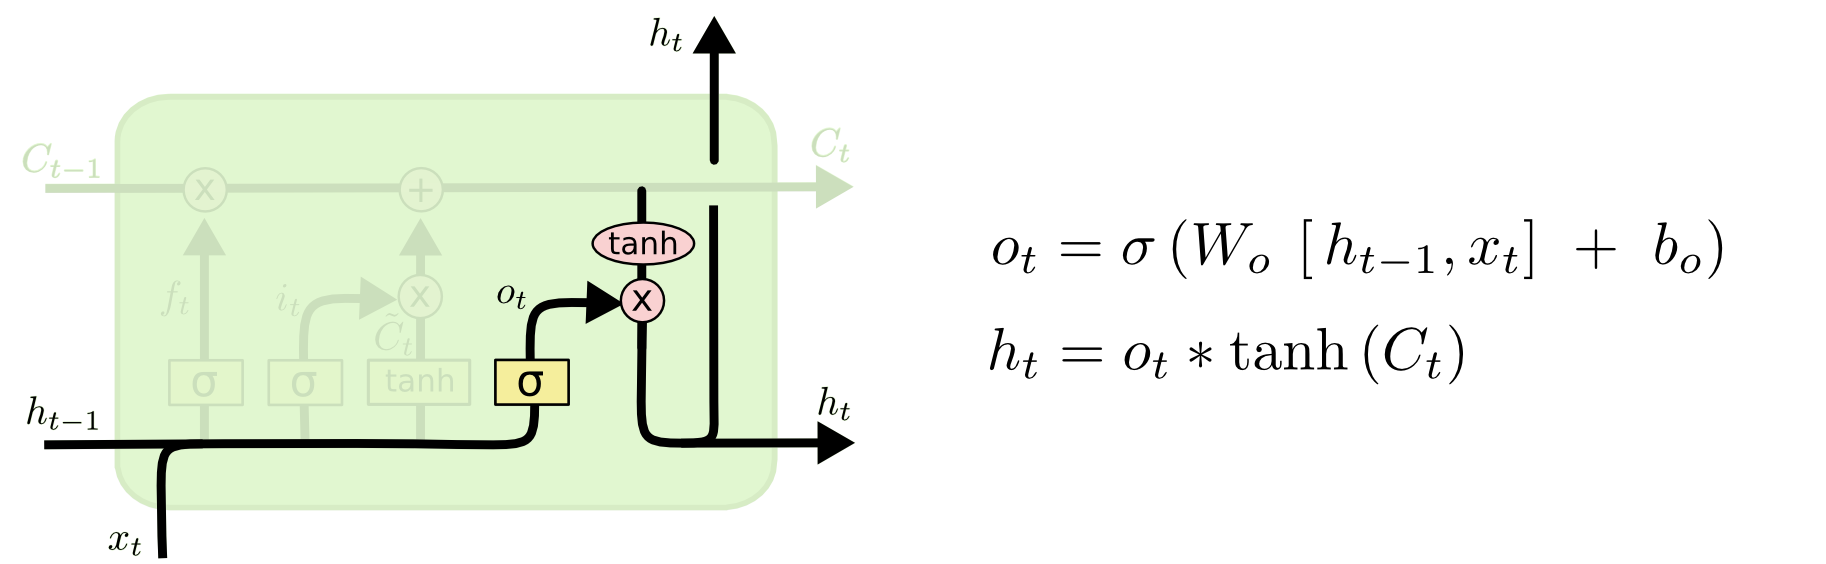
\includegraphics[width=0.7\textwidth]{Figures/LSTM3-focus-o.png}
	\caption[Output Gate.]{Output Gate.}
	\label{LSTM3-focus-C.png} 
\end{figure}
\end{itemize}
\subsubsection{Ưu điểm của LSTM}
LSTM là một bước lớn trong việc sử dụng RNN. Ý tưởng của nó giúp cho tất cả các bước của RNN có thể truy vấn được thông tin từ một tập thông tin lớn hơn. Ví dụ, nếu bạn sử dụng RNN để tạo mô tả cho một bức ảnh, nó có thể lấy một phần ảnh để dự đoán mô tả từ tất cả các từ đầu vào. Bằng chứng là Xu, et al. (2015) đã thực hiện được chính xác việc này. Hiện nay cũng đã có nhiều kết qua thực sự rất thú vị được chú ý và dường như có nhiều kết quả hơn chúng ta vẫn biết.
LSTM có những ưu điểm quan trọng áp dụng vào bài toán nhận diện hành động con người và xử lý chuỗi thời gian 
\begin{itemize}
    \item LSTM có khả năng lưu trữ thông tin lâu dài và xử lý các chuỗi dữ liệu dài và phức tạp hơn so với các kiến trúc mạng nơ-ron tái phát khác như mạng Elman hay mạng Jordan.
    \item LSTM được sử dụng để giải quyết các vấn đề trong xử lý ngôn ngữ tự nhiên như: phân loại văn bản, dịch máy, sinh văn bản tự động, tổng hợp giọng nói, và xử lý dữ liệu ngôn ngữ tự nhiên khác.
    \item LSTM có thể được sử dụng để giải quyết các vấn đề trong xử lý âm thanh và hình ảnh như: nhận dạng giọng nói dạng (voice recognition), phân loại hình ảnh, nhận diện khuôn mặt, phát hiện đối tượng và các ứng dụng khác trong lĩnh vực thị giác máy tính.
\end{itemize}

\section{Các thư viện sử dụng}
\subsubsection{Thư viện Numpy}
Thư viện NumPy (Numerical Python) là một thư viện Python phổ biến được sử dụng để làm việc với mảng đa chiều và các phép toán số học trên chúng. NumPy cung cấp một cấu trúc dữ liệu mảng mạnh mẽ và các hàm tiện ích để thực hiện các phép toán số học, xử lý mảng và thao tác trên dữ liệu số.
Dưới đây là một số khái niệm và tính năng chính của NumPy:
\begin{itemize}
	\item Mảng NumPy (ndarray): Mảng NumPy là cấu trúc dữ liệu chính trong NumPy, cho phép lưu trữ và xử lý các mảng đa chiều. Mảng NumPy có kích thước cố định và các phần tử trong mảng cùng kiểu dữ liệu.
	
	\item Các phép toán số học: NumPy cung cấp các hàm và toán tử cho phép thực hiện các phép toán số học trên mảng như cộng, trừ, nhân, chia, lũy thừa, căn bậc hai, logarit...
	
	\item Truy cập phần tử: Bạn có thể truy cập và thay đổi giá trị các phần tử trong mảng NumPy bằng cách sử dụng chỉ mục và cắt mảng (slicing).
	
	\item Hàm toán học và thống kê: NumPy cung cấp nhiều hàm toán học và thống kê tiện ích như min, max, mean, sum, std,... để thao tác trên mảng.
	
	\item Hàm điều kiện: NumPy cung cấp các hàm và phương thức cho phép kiểm tra và lựa chọn các phần tử trong mảng dựa trên các điều kiện như np.where, np.logical$\_$and, np.logical$\_$or,...
	
	\item Thao tác trên mảng: NumPy cung cấp các hàm và phương thức để thực hiện các phép biến đổi mảng như reshape, transpose, flatten, concatenate,...
	
	\item Tích hợp C/C++: NumPy cho phép tích hợp mã C/C++ vào mã Python thông qua giao diện C API của nó, giúp tăng tốc độ xử lý các phép toán số học.
	
	\item NumPy được sử dụng rộng rãi trong nhiều lĩnh vực như khoa học dữ liệu, máy học, tính toán khoa học, xử lý ảnh và âm thanh, mô phỏng vật lý,... Thư viện này là một phần quan trọng của hệ sinh thái Python cho tính toán số và xử lý dữ liệu.
\end{itemize}

\subsubsection{Thư viện OpenCV}

Thư viện cv2 (OpenCV) là một thư viện mã nguồn mở được sử dụng rộng rãi trong xử lý ảnh và thị giác máy tính trong ngôn ngữ lập trình Python. OpenCV cung cấp nhiều chức năng và công cụ mạnh mẽ để xử lý, phân tích và trực quan hóa ảnh và video. Dưới đây là một số chức năng chính của thư viện cv2:

\begin{itemize}
	\item Đọc và ghi ảnh và video: OpenCV cung cấp các hàm để đọc và ghi các tệp tin ảnh và video từ các nguồn khác nhau, bao gồm ổ đĩa, camera,...
	
	\item Xử lý ảnh: OpenCV cung cấp nhiều chức năng để xử lý ảnh, bao gồm chuyển đổi màu sắc, cắt, xoay, thu phóng, lật, v.v. Bạn cũng có thể áp dụng các bộ lọc, làm mờ, lọc nhiễu, phát hiện cạnh và nhiều phép biến đổi khác cho ảnh.
	
	\item Xử lý video: OpenCV hỗ trợ xử lý video, bao gồm khung hình theo thời gian, trích xuất khung hình, ghi lại video và áp dụng các hiệu ứng video.
	
	\item Xử lý thị giác máy tính: OpenCV cung cấp các chức năng và thuật toán để phân tích và nhận dạng các đối tượng trong ảnh, bao gồm nhận dạng khuôn mặt, phát hiện vật thể, trích xuất đặc trưng, theo dõi đối tượng,...
	
	\item Xử lý điểm ảnh: OpenCV cho phép bạn truy cập và chỉnh sửa các điểm ảnh trực tiếp, bao gồm xử lý pixel, tạo hiệu ứng đồ họa và thực hiện các phép tính điểm ảnh phức tạp.
	
	\item Hiển thị ảnh: OpenCV cung cấp các chức năng để hiển thị ảnh và video trực tiếp trên màn hình, tạo cửa sổ đồ họa và tương tác với ảnh.
\end{itemize}

Thư viện cv2 có tính ổn định, tốc độ xử lý nhanh và rất phổ biến trong cộng đồng xử lý ảnh và thị giác máy tính.

\subsubsection{Thư viện Tensorflow}

Thư viện TensorFlow là một thư viện mã nguồn mở phát triển bởi Google AI và được sử dụng rộng rãi trong lĩnh vực học máy và trí tuệ nhân tạo. TensorFlow cung cấp một cấu trúc dữ liệu gọi là "đồ thị tính toán" (computational graph) để biểu diễn và thực thi các phép tính toán số trên dữ liệu. Đồ thị tính toán trong TensorFlow bao gồm các nút (nodes) đại diện cho các phép tính toán và các cung (edges) đại diện cho luồng dữ liệu giữa các nút. Dưới đây là một số khái niệm và tính năng chính của TensorFlow:

\begin{itemize}
	\item Đồ thị tính toán (Computational graph): TensorFlow sử dụng đồ thị tính toán để biểu diễn và thực thi các phép tính toán. Đồ thị tính toán giúp tối ưu hóa và tận dụng được tính song song của phần cứng để thực hiện các phép tính nhanh chóng.
	
	\item Tensors: TensorFlow sử dụng cấu trúc dữ liệu tensor để lưu trữ và xử lý dữ liệu. Tensor có thể là một vector, ma trận, hay một mảng đa chiều với các phần tử cùng kiểu dữ liệu.
	
	\item Các lớp và phép tính: TensorFlow cung cấp một loạt các lớp và phép tính để xây dựng các mô hình học máy. Các lớp bao gồm các lớp mạng nơ-ron, lớp tích chập, lớp tổng hợp, lớp tái tạo,... Phép tính bao gồm các phép tính toán như cộng, trừ, nhân, chia, lũy thừa,...
	
	\item Tối ưu hóa và tạo mô hình: TensorFlow cung cấp các tối ưu hóa để tối đa hóa hiệu suất và tăng tốc độ huấn luyện mô hình. Ngoài ra, TensorFlow cũng cung cấp khả năng tạo và lưu trữ các mô hình đã huấn luyện để sử dụng sau này.
	
	\item Tích hợp và mở rộng: TensorFlow cho phép tích hợp và mở rộng với các công cụ và thư viện khác như Keras, scikit-learn, OpenCV, v.v. Điều này giúp thực hiện các tác vụ phức tạp và kết hợp các công cụ và thuật toán khác nhau.
	
	\item Tính tương thích và di động: TensorFlow hỗ trợ nhiều phiên bản và cung cấp tính tương thích đa nền tảng, cho phép chạy trên các thiết bị di động, máy tính cá nhân, máy chủ, và cụm máy tính phân tán.
\end{itemize}

TensorFlow là một công cụ mạnh mẽ trong lĩnh vực học máy và trí tuệ nhân tạo, cho phép xây dựng và huấn luyện các mô hình phức tạp và giải quyết các bài toán thực tế.

\subsubsection{Thư viện Sklearn}

Scikit-learn, hay còn được gọi là sklearn, là một thư viện mã nguồn mở phổ biến trong ngôn ngữ lập trình Python được sử dụng cho Machine Learning và Data Mining. Scikit-learn cung cấp nhiều công cụ và thuật toán tiện ích để xây dựng và đánh giá các mô hình học máy, phân tích dữ liệu và thực hiện các tác vụ tiền xử lý dữ liệu. Dưới đây là một số chức năng và tính năng chính của thư viện scikit-learn:

\begin{itemize}
	\item Cung cấp các thuật toán học máy tiêu chuẩn: Scikit-learn cung cấp các thuật toán học máy phổ biến như hồi quy tuyến tính, hồi quy logistic, máy vector hỗ trợ (SVM), cây quyết định, Random Forest, K-means clustering,... Các thuật toán này được triển khai một cách hiệu quả và dễ sử dụng.
	
	\item Tích hợp các công cụ tiền xử lý dữ liệu: Scikit-learn cung cấp nhiều công cụ tiền xử lý dữ liệu như chuẩn hóa dữ liệu, mã hóa biến định danh, xử lý giá trị thiếu, trích xuất đặc trưng,... Điều này giúp chuẩn bị dữ liệu cho việc huấn luyện mô hình.
	
	\item Đánh giá và tối ưu hóa mô hình: Scikit-learn cung cấp các phép đo và công cụ để đánh giá hiệu suất của mô hình học máy, bao gồm chia dữ liệu thành tập huấn luyện và tập kiểm tra, cross-validation, tính toán độ chính xác, độ phân loại, mất mát,... Ngoài ra, scikit-learn cũng cung cấp các công cụ tối ưu hóa để điều chỉnh các siêu tham số của mô hình.
	
	\item Tích hợp với các thư viện khác: Scikit-learn tích hợp tốt với các thư viện khác trong hệ sinh thái của Python như NumPy, Pandas và Matplotlib, tạo điều kiện thuận lợi cho xử lý dữ liệu và trực quan hóa kết quả.
\end{itemize}

Scikit-learn là một công cụ mạnh mẽ và phổ biến trong lĩnh vực Machine Learning, đặc biệt là trong các tác vụ phân loại, hồi quy và gom cụm dữ liệu. Với tư cách là một thư viện mã nguồn mở, scikit-learn đang tiếp tục được phát triển và cung cấp cập nhật mới để phục vụ cộng đồng Machine Learning ngày càng lớn.

\subsubsection{Thư viện Matplotlib}

Matplotlib là một thư viện trong Python được sử dụng để tạo và hiển thị đồ thị, biểu đồ, hình ảnh và các loại visualizations khác. Nó cung cấp các công cụ mạnh mẽ để tạo ra các biểu đồ chất lượng cao, giúp bạn trực quan hóa dữ liệu một cách dễ dàng và linh hoạt. Dưới đây là một số thành phần chính trong thư viện matplotlib:

\begin{itemize}
	\item pyplot: Giao diện API cơ bản của Matplotlib, cung cấp các hàm để tạo và tùy chỉnh đồ thị và biểu đồ.
	
	\item Figure: Đại diện cho một hình ảnh hoặc một tệp tin hình ảnh.
	
	\item Axes: Cung cấp các phương thức để tạo các đối tượng đồ thị như các trục, điểm, đường.
	
	\item Subplots: Cho phép tạo và quản lý nhiều đồ thị trong cùng một hình ảnh.
	
	\item Plot: Hàm để tạo các loại đồ thị và biểu đồ, bao gồm đồ thị đường (line plot), biểu đồ cột (bar plot), biểu đồ hộp (box plot), đồ thị điểm (scatter plot).
	
	\item Colorbar: Hiển thị thanh màu để giải thích giá trị của màu sắc trong đồ thị.
	
	\item Title, Label, Legend`: Cung cấp các phương thức để thêm tiêu đề, nhãn và chú giải vào đồ thị.
\end{itemize}

Matplotlib cũng hỗ trợ nhiều kiểu đồ thị và biểu đồ, cho phép bạn tùy chỉnh màu sắc, kích thước, kiểu đường, điểm, các đánh dấu trục, v.v. Thư viện này rất linh hoạt và mạnh mẽ, cho phép bạn tạo ra các visualizations phức tạp và tùy chỉnh chúng theo ý muốn.

\subsubsection{Thư viện Keras}

Keras là một thư viện mã nguồn mở cho Python được sử dụng để xây dựng các mô hình học máy và mạng nơ-ron. Nó được thiết kế để làm cho việc xây dựng mô hình học máy trở nên dễ dàng và nhanh chóng hơn. Keras có nhiều tính năng hữu ích, bao gồm:

\begin{itemize}
	\item Dễ dàng sử dụng: Keras được thiết kế để làm cho việc xây dựng mô hình học máy trở nên dễ dàng và trực quan hơn.
	
	\item Tích hợp với các thư viện tính toán số: Keras hỗ trợ các thư viện tính toán số như TensorFlow, Theano và CNTK, cho phép bạn chọn thư viện tính toán số phù hợp nhất cho dự án của mình.
	
	\item Hỗ trợ nhiều loại mô hình: Keras hỗ trợ nhiều loại mô hình, bao gồm mạng nơ-ron tiêu chuẩn, mạng nơ-ron tích chập và mạng nơ-ron tái tạo.
	
	\item Tích hợp với các công cụ tối ưu hóa: Keras cung cấp các công cụ tối ưu hóa để giúp bạn tìm kiếm các tham số tốt nhất cho mô hình của mình.
	
	\item Hỗ trợ các lớp và hàm kích hoạt tiêu chuẩn: Keras cung cấp các lớp và hàm kích hoạt tiêu chuẩn để giúp bạn xây dựng mô hình học máy nhanh chóng và dễ dàng.
\end{itemize}

Keras là một trong những thư viện phổ biến nhất cho việc xây dựng các mô hình học máy và mạng nơ-ron. 

\section{Thư viện MediaPipe}

Đây là một công cụ do google thiết kế ra, nó cung cấp nhiều tính năng cho các bài toán AI/ML chạy trên nhiều nền tảng khác nhau MediaPipe là tập hợp của một loạt các giải pháp Machine Learning đa nền tảng, có thể can thiệp được và cực kỳ lightweight.

Một số ưu điểm có thể kể tới của giải pháp này bao gồm:

\begin{itemize}
	\item Cung cấp một giải pháp inference nhanh chóng: Google khẳng định rằng bộ công cụ này có thể chạy ổn định trên hầu hết các cấu hình phần cứng thông dụng.
	
	\item Mã nguồn mở và miễn phí: Toàn bộ source code được công khai trên MediaPipe, người dùng hoàn toàn có thể sử dụng và tùy chỉnh trực tiếp để phù hợp với bài toán của mình.
	
	\item Dễ dàng cài đặt và triển khai: Việc cài đặt cực kỳ dễ dàng và tiện lợi, có thể triển khai trên nhiều nền tảng khác nhau như Mobile (Android/iOS), Desktop/Cloud, Web và IoT devices.
\end{itemize}

Hầu hết các bài toán nổi bật trong lĩnh vực Computer Vision - Thị giác máy tính, đều được Google cài đặt trong MediaPipe. Trong bài toán mình sẽ sử dụng Human Pose Estimation Mở rộng từ bài toán Hands Detection, Human Pose Estimation cung cấp một mô hình skeleton 3D cho cả cơ thể, với các khớp quan trọng được định nghĩa sẵn và được nối với nhau để tạo thành khung của người. Chiến thuật được đặt ra cho bài toán này tương tự như bài Hands Detection và Face Mesh. BlazeFace, một lần nữa, được sử dụng làm tư tưởng chính cho thuật toán xử lý bài này.

Các ứng dụng của mediapipe
\begin{itemize}
    \item Phát hiện khuôn mặt
    \item Tìm lưới khuôn mặt: dùng cho các ứng dụng biến đổi khuôn mặt như Tiktok
    \item Iris: tìm khoảng cách từ đồng tử của mắt đến camera mà không cần Depth webcam
    \item Detect cử chỉ bàn tay
    \item Tìm hình dáng của cơ thể
    \item Object detection , Box tracking
    \item Theo dõi chuyển động của vật thể
\end{itemize}

\section{Chỉ số đánh giá hiệu suất}

Để đánh giá phân loại ảnh được chính xác, các mô hình trong phần trước sữ được chạy bằng cách sử dụng bộ dữ liệu dưới dạng hình ảnh, vì vậy cần có sự điều chỉnh để nâng cấp độ chính xác của chúng. Đối với mỗi mô hình 3 kết quả điển hình được hiển thị trong CNN là:

\begin{itemize}
	\item Đồ thị độ chính xác (model ACC): ACC cho biết sự thay đổi độ chính xác của mô hình qua các vòng lặp/epochs trong quá trình huấn luyện.
	
	\item Đồ thị loss (model loss): Đồ thị loss biểu thị sự thay đổi của hàm loss của mô hình qua các vòng lặp hoặc epochs trong quá trình huấn luyện. Hàm loss tính toán sự sai khác giữa giá trị dự đoán của mô hình và giá trị thực tế.
	
	\item Confusion matrix: Về cơ bản, Confusion matrix thể hiện có bao nhiêu điểm dữ liệu thực sự thuộc vào một class, và được dự đoán là rơi vào một class. 
	
	\begin{figure}[h!]
		\centering
		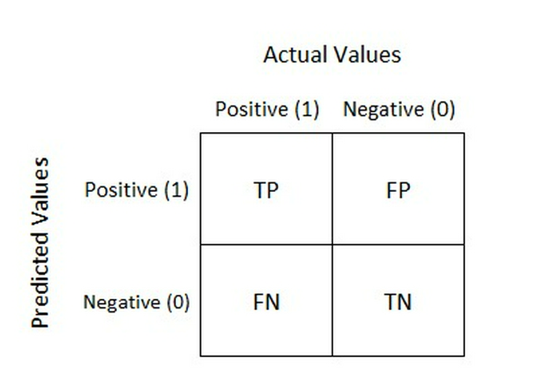
\includegraphics[width=0.7\textwidth]{cofusion.png}
		\caption[Confusion matrix.]{Confusion matrix.}
		\label{fig:cm} 
	\end{figure}

	\begin{itemize}
		\item TP (True Positive): Số lượng dự đoán chính xác.
		
		\item TN (True Negative): Số lương dự đoán chính xác một cách gián tiếp. Là khi mô hình dự đoán đúng một người không bị bệnh tức là việc không chọn trường hợp bị bệnh là chính xác.
		
		\item FP (False Positive - Type 1 Error): Số lượng các dự đoán sai lệch. Là khi mô hình dự đoán một người bị bệnh và người đó hoàn toàn khỏe mạnh.
		
		\item FN (False Negative - Type 2 Error): Số lượng các dự đoán sai lệch một cách gián tiếp. Là khi mô hình dự đoán một người không bị bệnh nhưng người đó bị bệnh, tức là việc không chọn trường hợp bị bệnh là sai. 		
	\end{itemize}
	$\Longrightarrow$ Từ 4 chỉ số TP, TN, FP, FN, ta có 4 chỉ số để đánh giá mức độ tin cậy của một mô hình:
\end{itemize}

\begin{itemize}
	\item Accuracy: Được tính bằng cách chia tổng số dự đoán đúng cho tất cả các dự đoán.
	
	\begin{figure}[h!]
		\centering
		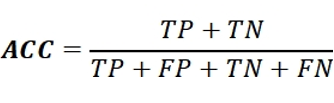
\includegraphics[width=0.45\textwidth]{acc1.png}
		\caption[Accuracy.]{Accuracy.}
		\label{fig:acc} 
	\end{figure}
		
	\item Precision: Trong tất cả các dự đoán Positive được đưa ra, bao nhiêu dự đoán là chính xác.
	
	\begin{figure}[h!]
		\centering
		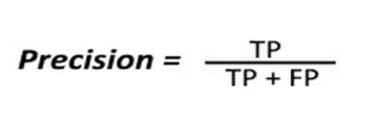
\includegraphics[width=0.6\textwidth]{precision.png}
		\caption[Precision.]{Precision.}
		\label{fig:precision} 
	\end{figure}
	
	\item Recall: Trong tất cả các trường hợp Positive, bao nhiêu trường hợp đã được dự đoán chính xác.		
	
	\begin{figure}[h!]
		\centering
		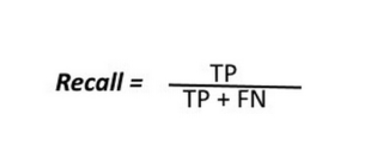
\includegraphics[width=0.6\textwidth]{recall.png}
		\caption[Recall.]{Recall.}
		\label{fig:recall} 
	\end{figure}

	\item F1-Score: Dùng để đánh giá mức độ tin cậy chung của mô hình
	
	\begin{figure}[h!]
		\centering
		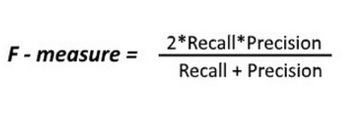
\includegraphics[width=0.6\textwidth]{score.png}
		\caption[F1-Score.]{F1-Score.}
		\label{fig:score} 
	\end{figure}
\end{itemize}








